\section{Durchführung}
\label{sec:Durchführung}

\begin{figure}
    \centering
    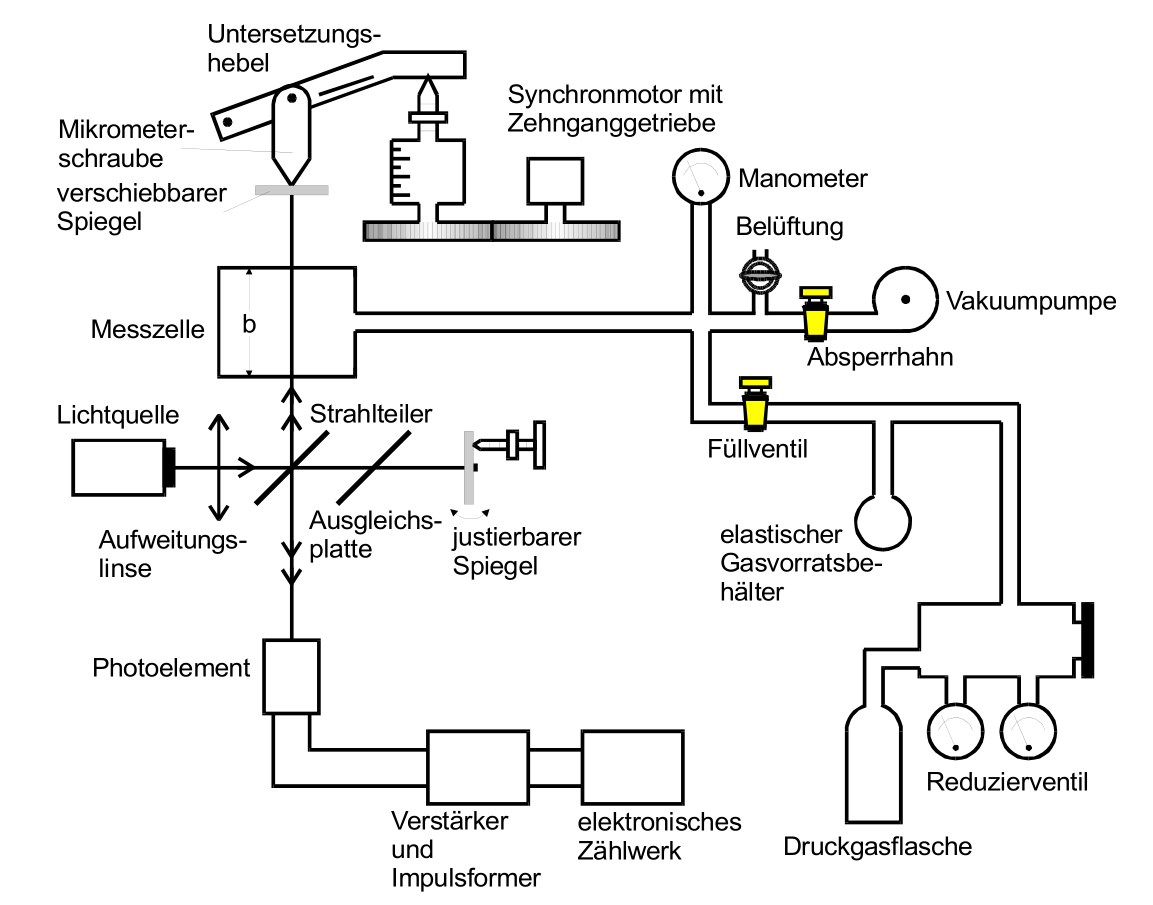
\includegraphics[width=12cm]{data/abb4.png}
    \caption{Darstellung der Messapparatur. \cite{sample}}
    \label{fig:abb4}
\end{figure}
\FloatBarrier

Vor der Messung muss der Aufbau noch justiert werden.
Die beiden hellsten Strahlen aus dem Interferrometer vom Laser sollen zur Deckung gebracht werden.
Dazu wird der verstellbare Spiegel so eingestellt, dass die beiden Strahlen auf eine Hilfsscheibe vor dem Detektor genau zur Deckung gebracht werden.
Sodann wird das Photoelement als Detektor auf die passende Höhe eingestellt, sodass das Interferenzbild genau parallel in den Schlitz trifft.
\\
Jetzt ist alles justiert und die Messung kann beginnen.
Dazu wird der verschiebbare Spiegel mit einem Synchronmotor und einer Mikrometerschraube verschoben.
Es wird die Spiegelverschiebung $d$ notiert, nach welcher mindestens 3000 Interferenzen vom Photoelement registriert wurden, sowie die exakte Anzahl $z$ von Interferenzen.
Diese Messung wird zehn mal wiederholt.
\\
Um den Brechungsindex von Luft zu messen, wird der verschiebbare Spiegel in Ruhe gelassen.
Die Messzelle wird auf ein Druck $p$ evakuiert, welcher notiert wird.
Beim Wiedereinlassen der Luft werden erneut Interferenzen gezählt, deren Anzahl $z$ ebenfalls notiert wird.
Der sich dann einstellende Druck wird als Normaldruck $p_0$ notiert.
Diese MEssung wird auch zehn mal wiederholt.
